\chapter{Dataset}
\label{chapter:dataset}

In this chapter we will provide information about the datasets we used in our research. We will describe how we obtained a labeled dataset for training and also mention the weaknesses associated with this dataset. We will take a look at the important properties of the logs. 
We will also discuss some known anomaly scenarios that can occur in the system logs, and we will go through the dataset in which they are captured. 
We use the anomalies to validate our models. A validation dataset that contains anomaly-free data will also be described. 

All datasets contain log traces collected from multiple microservices comprising the Motorola SmartConnect Cloud Infrastructure Engineering development environments.
To obtain the logs, we developed a pipeline (the details of the pipeline are described in Chapter~\ref{data_collection}) that connects to the system, collects logs, and preprocesses them into such a form that the data can be passed to selected machine learning algorithms or plotted.
More about the preprocessing step can be found in Chapter \ref{methodology}.

\section{Datasets}
\label{dataset}
The data we feed machine learning models with makes a big difference. Therefore, we need to look at what data we can collect at a high level from the system and what properties an individual log entry has.

The anomaly detection task can be reformulated as a classification problem with two classes: \textit{negative (anomaly)} class and \textit{positive (anomaly-free)} class. 

\textit{Negative} or \textit{normal} class is a category of a dataset that is free of anomalies and represents the expected (or normal) behaviour of a system that produces these logs. Negative data samples are labeled as $0$. The class \textit{Positive}, \textit{anomalous}, or \textit{abnormal} is the target class we are interested in. It is assigned to log sequences that contain anomalies as $1$. The goal is to train the classifier to distinguish between positive and negative samples.

Motorola Solution's policy for storing historical data is that we have logs available at any point in time from $30$ days ago to this point in time. The stored interval may at times become even smaller if the amount of persisted logs exceeds a limit.

In Motorola, the development environment is further divided into two subsections that we have access to. 
Let's call them \textit{experimental} and \textit{stable}. 

The \textit{stable} environment is synchronized with all the master branches of the source code. It is used to perform extensive testing of the system every night. 

On the other hand, the \textit{experimental} environment is used by the developers to deploy and explore side (or feature) branches during the day.

For confidentiality reasons, we do not have logs of the \textit{production} environment available. This is one of the major drawbacks, as it can be assumed that they contain different traffic. It can also be assumed that the distribution of anomalies in \textit{production} environment is different from both \textit{experimental} (more anomalies, some related to ad hoc deployment) and \textit{stable} (fewer anomalies, less traffic). In general, the development environment produces huge amounts of data, thousands of log messages per minute.

Next, we provide a detailed description of the characteristics of each dataset and how they were obtained. See Table \ref{table:datasets} for a summary of all datasets used in this work.

\subsection{Dataset Daily} 
This dataset reflects the \textit{experimental} region of the development environment. In such an environment, it is natural (or even desirable) for anomalies to occur.

We refer to the dataset of system logs produced by the region as the \textit{Daily} dataset, and may also refer to it as \textit{mixed}, since it will contain both positive and negative data samples. 
The system is active during a working day when developers are testing new features. The amount of logs varies greatly depending on the team's tasks. 
However, we are talking about tens of thousands of log messages per hour, even when the system is idle.

Unfortunately, such a dataset is not labeled, as experts would have to go through millions of lines of unstructured log messages to obtain the labels.

\subsection{Dataset Nightly}
At night, the system we are experimenting with goes through tests in the \textit{stable} region. This phase of health check of the system involves mimicking the normal behaviour of the telecommunications system. All the necessary infrastructure setup takes place and simulations of calls between groups of push-to-talk radios are performed. 
These tests are run again each night as part of the nightly test suite. 
Typically, the test pipeline lasts about 7 hours and produces about 2 million log messages.

If the nightly tests all pass, the data collected should either be completely free of anomalies, or contain only a very small percentage of them. 
Therefore, we assume that the data collected during the nightly testing phase, if passed successfully, will contain a large majority of negative data samples and represent normal anomaly-free behaviour of the system. This statement relies heavily on the assumption that the functionality of the system is well covered by the tests (the relationship of our approach to anomaly detection and test code coverage is discussed in detail in Section~\ref{code_coverage}). 

Therefore, for our use case, we can also interchangeably refer to the dataset \textit{Nightly} as \textit{negative} or \textit{normal} dataset.

Therefore, the logs collected at night by such a system should be suitable candidates for one-class classification algorithms as well as generate a labeled dataset for testing purposes, which we will explain later in this chapter.

However, the data generated by the system during nightly testing is slightly different from the live production environment. The main difference is that the scenarios generated by the test suite are serialized, meaning that there is at most one call at any given time. 

On the other hand, in the live production environment, there is no limit to the number of radio broadcasts at a time. Therefore, the logs of the production environment can contain much higher counts of some events.

Although this could be argued as a weakness of our nightly dataset, as described windowing operation of our preprocessing phase in Chapter~\ref{methodology}, we will always consider a sequence of logs and the number of event types in that log sequence in a fixed time window. Therefore, we believe that the final feature representation passed to the ML algorithm should be very similar, even though the data will look different with respect to individual log entries.

Since it is incredibly difficult to obtain labels in log data, we decided to use the Nightly data, despite its potential drawbacks and slightly artificial nature.

The Nightly data contains logs from the night of January 24, 2021.

\subsection{Dataset Nightly Test}
This dataset was collected in the same way as the Nightly and should meet all the properties, but it was recorded on a different day. Therefore, the timing is different and the tests are examining a different version of the SmartConnect system source code.

We use Nightly Test mainly to show that a similar distribution of arbitrary records collected during any nightly testing can be assumed.

Nightly Test contains logs from the night of January 22, 2021.

\subsection{Dataset Anomalies}

This dataset contains versions of the two anomaly scenarios described later in Section~\ref{anomaly_types}. 
The anomalies were achieved by killing Kubernetes Pods, which is responsible for the correct operation of a particular service type. 
At the same time, users were trying to establish, or were in a call.

This dataset captures a total of 23 instances of anomaly scenarios and was created by merging logs from two days - January 25 and 28, 2021.

\subsection{Dataset Glostrup Calling}

In contrast, the Glostrup Calling dataset consists of anomaly-free calls between Motorola Solutions two-way radios. 
The \textit{experimental} environment was set so that nothing else interferes with the calls. Therefore, the resulting logs can be considered as \textit{normal} data.

The trace records several calls that were carried out during 8 minutes on February 3, 2021.

\section{Dataset Test with Labels} 
\label{section:testset}
Unsupervised learning does not require data to be labeled to detect anomalies, as it assumes that the majority of data points are normal.  This is very beneficial in our situation where it is extremely difficult to obtain labeled data. However, the lack of labels poses a difficulty when it comes to the model evaluation phase.

Unlike supervised learning, where one can directly compare predictions with actual labels to assess the quality of the machine learning model, there is no way to do this in unsupervised learning.

In our work, the majority of the data is unlabeled data. To validate the proposed approaches, we had to develop the test dataset ourselves.

To get a better idea of what kind of data constitutes a manually created test dataset, we provide a pie chart of the test set composition in Figure \ref{fig:testset-composition}. It is important to note that the number $131$ represents the amount of extracted log sequence, so the number of underlying log message samples is much higher.

Determining the negative class representation is trivial. As we mentioned earlier in this chapter, we consider the Nightly data from the testing phase as normal data samples. To create the normal part of the dataset, we collect another set of data from the testing phase that was previously unseen in the training phase. 

On the other hand, positive samples must be manually labeled. To avoid label assignment errors, we introduce some known anomaly scenarios that are expected to occur in our real dataset. These scenarios can be reproduced, we can collect the data and label them as anomalies. 

This is not an ideal test dataset, but not all anomalies are known and can be sourced. It provides a reasonable tool to measure how well our models are performing. We will also test the models with only normal data to detect false positives. 

\begin{figure}[h]
    \centering
    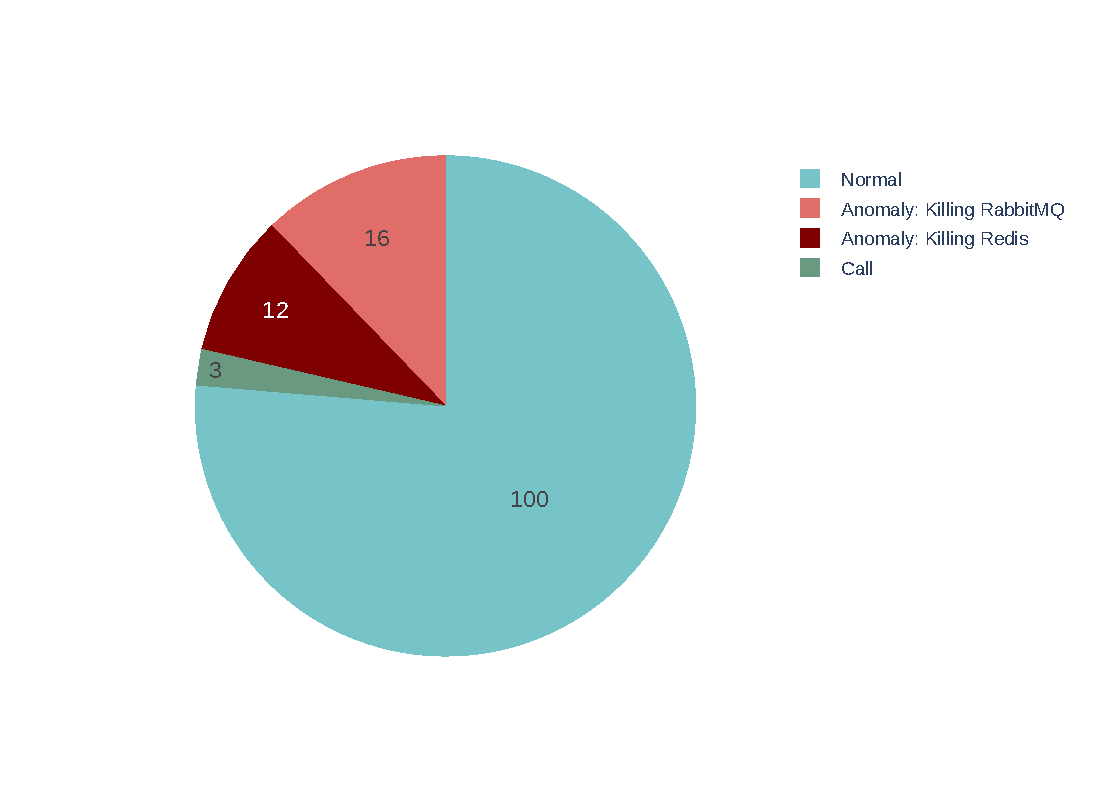
\includegraphics[width=0.8\textwidth]{img/testset-composition.pdf}
    \caption{Testing dataset composition. A manually collected and labeled dataset consists of 131 log sequences, where each log sequence was collected within a two-minute time window. The value in each section of the pie chart indicates the number of log sequences of each type of log message it contains. The "Normal" and "Call" sections of the pie chart both represent normal, anomaly-free behaviour, while " Killing RabbitMQ" and "Killing Redis" are anomalies.}
    \label{fig:testset-composition}
\end{figure}

\begin{table}[!h]
\centering
\resizebox{\textwidth}{!}{\begin{tabular}{@{}lcr@{}}
\toprule
\textbf{Dataset Name} & \textbf{Log Entries}       & \textbf{Size}  &\textbf{Time Span}  \\ \toprule
\textcolor{customDarkBlue}{\textbf{Daily}}           & $539\,372$    & $2.84$ GB     & \footnotesize{ 26/1/2021 6:00  -  26/1/2021 21:00 }     \\ \midrule
\textcolor{customDarkBlue}{\textbf{Nightly}}         & $1\,362\,004$ & $4.24$ GB     &  \footnotesize{24/1/2021 21:00  -  25/1/2021 3:50}      \\ \midrule
\textcolor{customDarkBlue}{\textbf{Nightly Test}}    & $1\,373\,919$ & $4.47$ GB     &  \footnotesize{22/1/2021 21:00  -  23/1/2021 3:43}      \\ \midrule
\textcolor{customDarkBlue}{\textbf{Anomalies}}       & $805\,614$    & $3.6$ GB      & \footnotesize{ 25/1/2021 15:40  -  25/1/2021 17:00,  28/1/2021 15:25  -  28/1/2021 16:00}    \\ \midrule
\textcolor{customDarkBlue}{\textbf{Glostrup Calling}}    & $1904$    & $15.82$ MB    &  \footnotesize{3/2/2021 9:40  -  3/2/2021 9:47} \\
\bottomrule
\end{tabular}}
\caption{Summary of all the log datasets we worked with in our research on anomaly detection.}
\label{table:datasets}
\end{table}

\section{Log Properties}
The services record 33 properties per single log entry. Of the 33 log properties, we chose to consider only \texttt{msg} and \texttt{timestamp}, as the others (such as the name of the Kubernetes pod, the process ID of the service generating the log, etc.) are too specific. For the full list of the individual log properties see Appendix~\ref{appendix:log-properties}).
Including fewer predictor variables should generally avoid overfitting, make the final model more transparent, and make debugging easier.
Therefore, to obtain as general a solution as possible, we restrict ourselves to these two predictors.

\subsection{Format of Log Properties}
Messages are strings and we assume that they follow the logic we described in Section~\ref{log_template_mining} on log template mining. In other words, we assume that they are generated by code in such a way that they can be thought of as a product of constant and variable parts. Consequently, log messages can be further categorized using event types.

Timestamps have the format of \texttt{YYYY-MM- DD'T'HH:mm: SS.sss'Z'}. The format string indicates that the year (YYYY) is a four-digit number padded with zeros, the month (\texttt{MM}), the day (\texttt{ DD }), the hour (\texttt{HH}), the minutes (\texttt{mm}) and the seconds (\texttt{ SS }) are two-digit zero padded numbers and the milliseconds (\texttt{ssss}) are a three-digit number filled with zeros. The time part is separated from the date by a single \texttt{T} character and the entire timestamp ends with a letter \texttt{Z}.

\section{Types of Anomalies}
\label{anomaly_types}
In this section, we present a set of known anomalies that we will trace in order to test our solution.
We will benchmark our approaches and models to these known anomalies, which can be easily simulated and reproduced. 
However, the goal is to also detect anomalies that we are not aware of.
In other words, we also want to identify anomalous scenarios that appear for the first time in the production environment and do not appear in our training and testing dataset.

\subsection{Cache Outage}
In this anomaly, a cache storage that orchestrates the call logic is taken down and the radios that are in a call at that moment bonk because they cannot communicate with each other.
In response, the storage service automatically restores itself, usually in no more than 2 seconds. After that, broadcast should continue.

As mentioned in Section~\ref{architecture:caching} about caching in Motorola SmartConnect, Redis is used for caching, so we can also call this anomaly \textit{ Killing Redis } or similar.

\subsection{Message Broker Out of Service}
Similarly, an important entity in the SmartConnect microservices system is the message broker that enables inter-service communication. In this scenario, all brokers are terminated, therefore the microservices network is disrupted and messages cannot be forwarded until the brokers are restored.

Section~\ref{architecture:messaging} discusses again how messages are forwarded in SmartConnect's microservices architecture. RabbitMQ is the specific message broker that is used, so we can refer to this anomaly in the text as \textit{Killing RabbitMQ}.

% https://pure.tue.nl/ws/portalfiles/portal/142685995/sci_2019_Lomagin_Egor.pdf